\documentclass[10pt]{article}
\usepackage[margin=1.6cm]{geometry}
\usepackage{graphicx}
\usepackage{booktabs}
\usepackage{array}
\usepackage{amsmath}
\usepackage{enumitem}
\usepackage{titlesec}
\usepackage{xcolor}
\usepackage[colorlinks=true, linkcolor=blue, urlcolor=blue, citecolor=blue]{hyperref}
\usepackage{caption}
\usepackage{float}

\titlespacing*{\section}{0pt}{6pt}{3pt}
\titlespacing*{\subsection}{0pt}{5pt}{2pt}
\setlist{nosep, leftmargin=1.4em}
\captionsetup{font=small, labelfont=bf}
\renewcommand{\arraystretch}{1.05}

\title{\vspace{-1.3cm}\large Assignment 3: Benchmarking Approximate Nearest Neighbour Search}
\author{KSPSVLN Siddardha Kumar Kavuri \ (2025201061) \\ \small \href{https://github.com/siddardhakumar2003/Information-Retrieval-Extraction/tree/main/Assignment-3}{Code repository (GitHub)}}

\begin{document}
\maketitle
\vspace{-0.9cm}

\section*{Methodology and environment}
\small
Datasets: SIFT (1M, 128d, Euclidean) and GloVe-100 (1.18M, 100d, cosine $\to$ L2-normalised and
treated as Euclidean), both from ann-benchmarks. Queries were split 5000/5000: the first 5000
(``tune'') were used only for a coverage check that the swept parameter grid reaches recall
$\geq 0.95$; the last 5000 (``final'') are the only queries used for every reported number, to
avoid selection bias on the tuning split. Exact recall@10 was verified against the datasets'
stored ground truth (recall $=1.0000$ on both). All search timing is single query at a time,
single thread, median of 3 repeats (1 repeat in \texttt{--quick} mode).

All four parts ran on a single machine: an IIIT-H Ada cluster node (Intel Xeon E5-2640 v4,
40 cores, 131.9\,GB RAM, Python 3.10.12), CPU-only for search (IVF training used GPU
acceleration where available, never benchmarked search). Library versions:
\texttt{faiss-cpu 1.15.1}, \texttt{hnswlib 0.8.0}, \texttt{numpy 2.2.6}, \texttt{pandas 2.3.3}.
Full specs/versions are in \texttt{results/environment.txt}. Because the full (non-\texttt{--quick})
sweep exceeds Ada's 6-hour job wall-clock limit in one run, the four parts were submitted as
separate jobs on the same node/account over several days rather than one continuous job; every
reported number nonetheless comes from this one machine.

\section*{Part 1: Exact baseline}
\begin{center}
\small
\begin{tabular}{lccccc}
\toprule
dataset & build time (s) & recall@10 & single-query QPS & batched QPS (1 thr) & batched QPS (40 thr) \\
\midrule
SIFT (1M, 128d)     & 0.41 & 1.0000 & 27.3 & 259.1 & 395.5 \\
GloVe (1.18M, 100d)  & 0.31 & 1.0000 & 28.6 & 268.7 & 369.2 \\
\bottomrule
\end{tabular}
\end{center}
\textbf{Why batching is so much faster, even at one thread:} a single \texttt{search()} call
amortises the fixed Python/FAISS call overhead (argument marshalling, GIL handoff, BLAS call
setup) across all 5000 queries instead of paying it once per query, and lets FAISS issue one
large, cache-friendly matrix--matrix distance computation (effectively a GEMM) instead of 5000
separate matrix--vector calls, which is far more efficient per floating-point operation on modern
CPUs. The further jump from 1 to 40 threads comes from FAISS parallelising that batched distance
computation itself across cores -- a benefit a single one-row query cannot use, since there is
nothing to split across threads (the gain is sub-linear in core count because only the
distance-computation inner loop parallelises; call overhead and result aggregation stay serial).

\section*{Part 2: Benchmarking HNSW, IVF-Flat, IVF-PQ}

\begin{figure}[H]
\centering
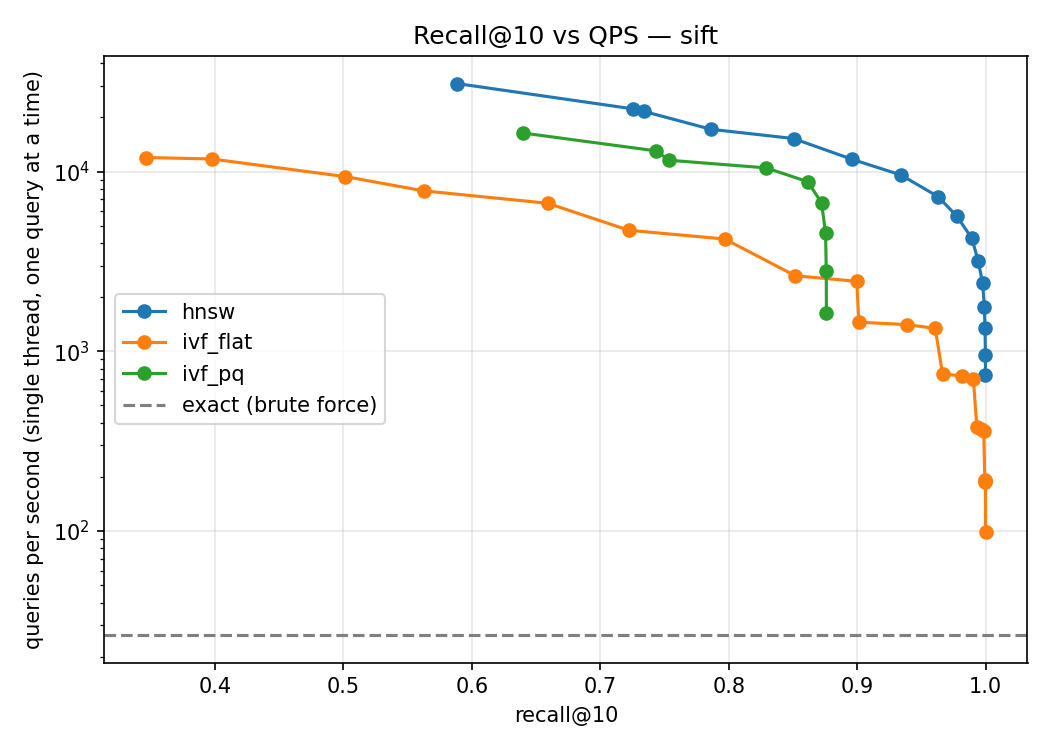
\includegraphics[width=0.49\linewidth]{../results/figures/part2_recall_vs_qps_sift.png}
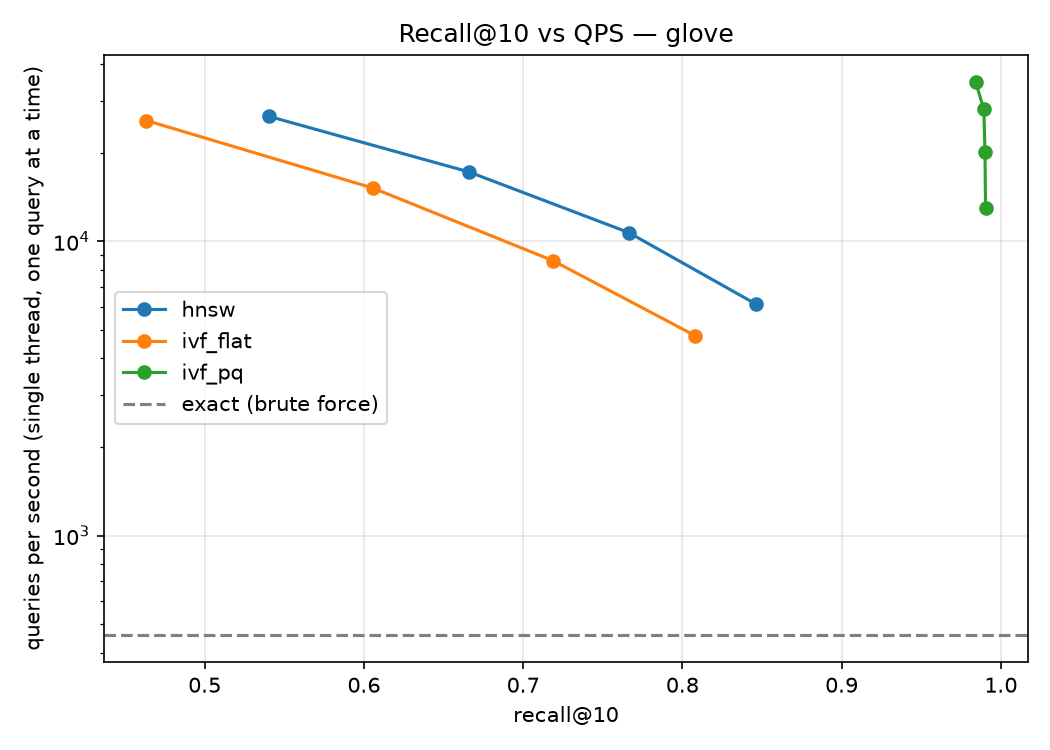
\includegraphics[width=0.49\linewidth]{../results/figures/part2_recall_vs_qps_glove.png}
\caption{Recall@10 vs.\ queries/sec (best trade-off curve per index), SIFT (left) and GloVe-100 (right). Dashed line: exact baseline QPS.}
\end{figure}

\begin{table}[H]
\centering\small
\begin{tabular}{l c c c c}
\toprule
 & \multicolumn{2}{c}{SIFT: QPS @ recall} & \multicolumn{2}{c}{GloVe: QPS @ recall} \\
index & 0.90 & 0.95 & 0.90 & 0.95 \\
\midrule
HNSW     & 9{,}704 & 7{,}121  & 1{,}437 & 428 \\
IVF-Flat & 1{,}472 & 1{,}369  & 476   & 245 \\
IVF-PQ   & not reached & not reached & 17{,}013 & 13{,}043 \\
\bottomrule
\end{tabular}
\hspace{0.5cm}
\begin{tabular}{l c c c}
\toprule
\multicolumn{4}{c}{at recall $\geq 0.95$: build time (s) / bytes-per-vector} \\
index & SIFT build (s) & SIFT B/vec & GloVe build (s) / B/vec \\
\midrule
HNSW     & 53.1 & 597.2 & 226.9 / 676.3 \\
IVF-Flat & 4.7  & 520.3 & 4.5 / 408.2 \\
IVF-PQ   & not reached & -- & 58.2 / 13.8 \\
\bottomrule
\end{tabular}
\caption{Left: queries/sec at recall@10 $\geq$0.90 / 0.95. Right: build time and memory at recall $\geq 0.95$ (raw vectors: 512\,B/vec for SIFT, 400\,B/vec for GloVe).}
\end{table}

\textbf{Why IVF-PQ fails to reach 0.95 on SIFT:} across all 4 swept build configs
(nlist $\in\{500,2000\}\times$ m\_subvectors $\in\{8,16\}$), recall \emph{plateaus} between 0.81
and 0.88 and stops improving even as \texttt{nprobe} is pushed to scan the entire index
(nprobe=500) -- e.g.\ nlist=2000, m=8 climbs from 0.63 at nprobe=1 to 0.876 at nprobe=16 and then
is flat to nprobe=512. This is not a search-effort problem: the asymmetric distance computation
itself is capped by the product-quantiser's reconstruction error, which SIFT's heavier-tailed
128-d descriptor distribution exposes more than GloVe's lower-dimensional, L2-normalised
100-d vectors (where IVF-PQ reaches 0.955 and, notably, becomes the \emph{fastest} index overall).

\section*{Part 3: Scaling experiment (standard data)}
\textbf{Hypothesis} (committed to \texttt{hypothesis.md} before running): exact QPS degrades
roughly linearly with $N$ ($\sim$10$\times$ drop from 100K$\to$1M); HNSW degrades much more
slowly ($\sim\log N$); IVF-Flat (nlist $\propto\sqrt{N}$) falls in between, $\sim\sqrt{N}$.

\begin{figure}[H]
\centering
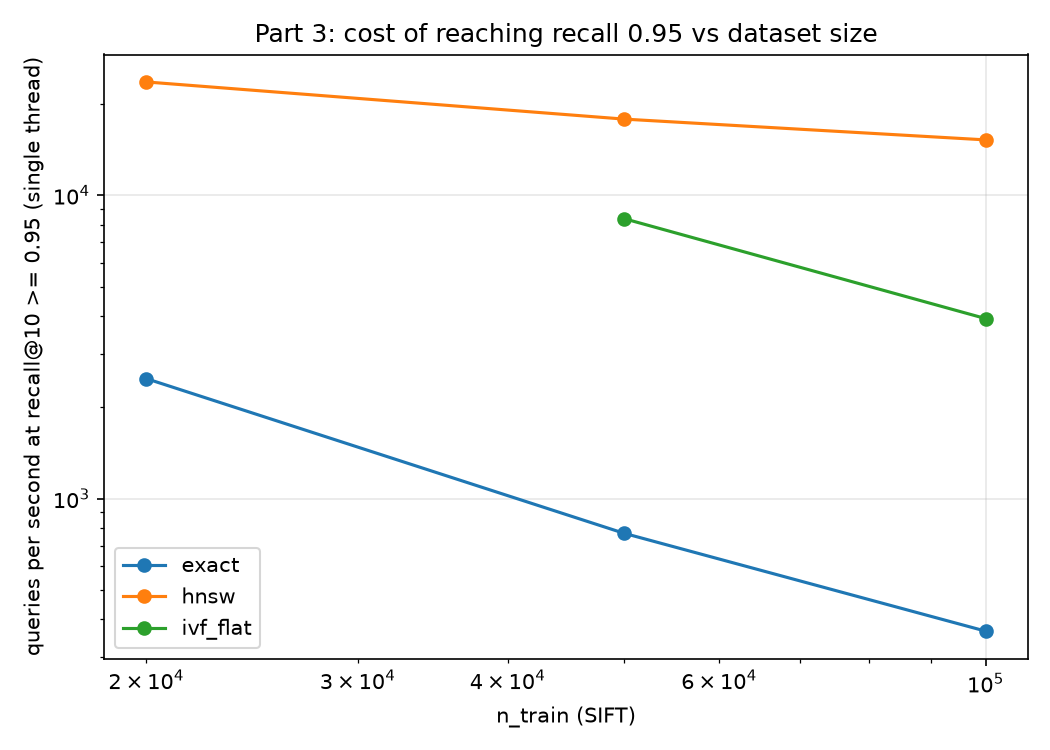
\includegraphics[width=0.52\linewidth]{../results/figures/part3_scaling_qps_at_recall95.png}
\caption{QPS at recall@10 $\geq$0.95 vs.\ SIFT training-set size (log--log).}
\end{figure}

\textbf{Result: hypothesis supported.} Exact: 237.2$\to$80.2$\to$26.6 QPS (100K/300K/1M) -- an
8.9$\times$ drop over 10$\times$ N, close to linear. HNSW: 11{,}978$\to$10{,}092$\to$7{,}357 --
only a 1.6$\times$ drop, consistent with logarithmic growth in graph hops. IVF-Flat:
4{,}391$\to$2{,}434$\to$1{,}374 -- a 3.2$\times$ drop, almost exactly $\sqrt{10}\approx3.16$,
matching the $\sqrt{N}$ prediction. \textbf{Implication:} a benchmark run only at small $N$ would
understate how much HNSW's relative advantage over exact/IVF-Flat grows at real scale -- the
Part 2 headline numbers (measured only at 1M/1.18M) are a snapshot at one scale, not a
scale-invariant ranking.

\section*{Part 4: Dimensionality experiment (self-generated data)}
\textbf{Hypothesis} (committed before running): recall@10 at a \emph{fixed} search budget
(HNSW ef=40, IVF-Flat nprobe=8, both on i.i.d.\ uniform-random data, $N$=50{,}000 fixed) degrades
monotonically as dimensionality $d$ grows, because nearest/farthest-neighbour distances
concentrate (``curse of dimensionality''), weakening distance-based pruning; exact search is
unaffected since it never prunes.

\begin{figure}[H]
\centering
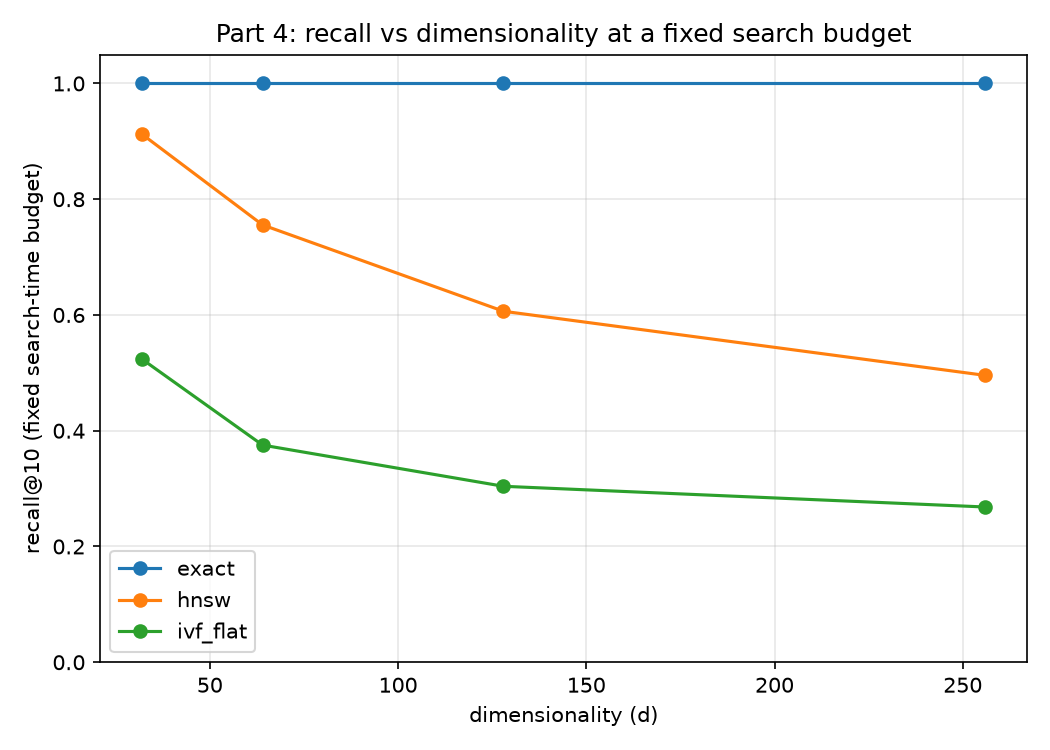
\includegraphics[width=0.46\linewidth]{../results/figures/part4_dimensionality_recall.png}
\caption{Recall@10 vs.\ dimensionality $d$ at a fixed search budget, uniform-random synthetic data.}
\end{figure}

\textbf{What changed:} $d \in \{32\text{ (control)}, 64, 128, 256\}$, all else fixed (N, seed,
HNSW/IVF-Flat config). \textbf{What happened:} recall falls monotonically for both indexes --
HNSW 0.815$\to$0.528$\to$0.350$\to$0.256, IVF-Flat 0.567$\to$0.379$\to$0.276$\to$0.216 -- while
exact stays at 1.000 throughout. \textbf{Mechanism:} as $d$ grows, the ratio of nearest- to
farthest-neighbour distance tends to 1 (distance concentration), so both HNSW's greedy graph
search and IVF-Flat's cluster-probe step can no longer reliably tell a true near neighbour from a
distractor at a fixed search budget -- more of the true top-10 falls outside the candidates the
fixed budget examines. \textbf{Supports hypothesis:} yes, cleanly and monotonically.
\textbf{Not tested:} whether \emph{increasing} the search budget (larger ef/nprobe) at high $d$
can recover the lost recall, and whether real (non-uniform, clustered) high-dimensional embeddings
degrade the same way -- uniform random data is close to a worst case for distance concentration.

\section*{Part 5: Discussion}
\textbf{1. Fastest index at recall 0.95 -- does the answer change between datasets?} Yes,
sharply. On SIFT, HNSW is fastest (7{,}121 QPS) by 5--6$\times$ over IVF-Flat, with IVF-PQ unable
to reach 0.95 at all. On GloVe, IVF-PQ is fastest (13{,}043 QPS), over 30$\times$ faster than
HNSW (428 QPS) on that dataset. The mechanism: GloVe-100's normalised, lower-dimensional vectors
compress well under product quantisation (13.8 bytes/vector, see Q2) and its angular geometry is
known to be harder for graph-based search -- GloVe has more near-duplicate/``hub'' points, which
means HNSW's greedy graph walk needs far more hops (lower ef efficiency) to reach the same recall
than it does on SIFT's more isotropic descriptor space. So the dataset's geometry, not just its
size, decides which index wins -- there is no single best index.

\textbf{2. Build time and memory cost; what does PQ trade off?} HNSW is by far the most
expensive to build (53--227s) because it constructs an explicit proximity graph with backlinks;
IVF-Flat is cheap to build (4.5--4.7s, just k-means + bucket assignment) since it does no graph
construction; IVF-PQ build time sits between the two (58s on GloVe) because it also runs a
k-means codebook training step on top of the IVF assignment. On memory, HNSW is the most
expensive per vector (597--676 B/vec, raw vectors plus the graph's adjacency lists), IVF-Flat
is close to raw-vector size (408--520 B/vec, just the original vectors plus a small list
overhead), and IVF-PQ is dramatically smaller (13.8 B/vec on GloVe -- a $\sim$49$\times$
reduction vs.\ HNSW) because it stores only compressed per-sub-vector codes instead of full
vectors. The trade PQ makes for that compression is a hard ceiling on achievable recall (Q2 of
Part 2) set by quantisation error, which no amount of extra search effort (nprobe) can overcome
-- seen directly in SIFT, where PQ plateaus around 0.88 regardless of how much of the index is
scanned.

\textbf{3. What do Parts 3 and 4 show about when headline numbers could mislead?} Part 3 shows
the Part 2 ranking (``HNSW beats IVF-Flat'') is not fixed -- it \emph{widens} with scale (HNSW's
QPS-at-recall-0.95 advantage over IVF-Flat grows from 2.7$\times$ at 100K to 5.4$\times$ at 1M), so
a small-scale benchmark would understate HNSW's real advantage at production scale. Part 4 shows
the opposite kind of risk: the Part 2 numbers were measured only at SIFT's native 128d / GloVe's
100d; at higher dimensionality (e.g.\ modern 768--1536d embedding models), the \emph{same} fixed
search budget that gave 0.95+ recall here could give well under 0.3 recall, because recall itself
-- not just speed -- degrades with dimensionality. Together: headline recall-vs-QPS numbers are
specific to one $(N, d)$ operating point and do not automatically transfer to a different scale or
embedding dimensionality without re-benchmarking.

\textbf{4. 150{,}000 vectors vs.\ 10 million, 100\,ms/query budget, 16\,GB RAM -- use ANN?}
Fitting a power law to the Part 3 exact-search points ($\text{QPS}\propto N^{-0.95}$, from
237.2 QPS at 100K to 26.6 QPS at 1M on the Ada machine) gives: at \textbf{150K} vectors, exact
QPS $\approx 161$, i.e.\ $\approx$6.2\,ms/query -- comfortably inside the 100\,ms budget, and
memory for raw 128-d float32 vectors is $\approx$77\,MB, negligible against 16\,GB. \emph{Use
exact search} -- it gives perfect recall with zero tuning and the budget is not binding at this
size, so ANN would only add complexity for no benefit. At \textbf{10M} vectors, the same fit
gives exact QPS $\approx 3.0$, i.e.\ $\approx$335\,ms/query -- over 3$\times$ the 100\,ms budget,
so exact search fails here and ANN is required. Memory at 10M is not the binding constraint for
either HNSW ($\approx$5.97\,GB at 597 B/vec) or IVF-Flat ($\approx$5.2\,GB at 520 B/vec) --
both fit well inside 16\,GB. Given 100\,ms is a very generous budget relative to the
sub-millisecond latencies HNSW/IVF-Flat already achieve at 1M (Part 2), the deciding factor is
recall and throughput headroom rather than the budget itself: \emph{use HNSW}, tuned to roughly
the ef that gave recall $\approx$0.97 on SIFT at 1M, since it dominates IVF-Flat on both recall
ceiling and QPS at recall 0.95 (7{,}121 vs.\ 1{,}369 QPS) for only $\sim$15\% more memory per
vector. If the scale were pushed further (e.g.\ 100M+, where 16\,GB would no longer hold HNSW's
graph) IVF-PQ's $\sim$14--100 B/vec compression would become the memory-forced choice instead,
accepting its lower recall ceiling.

\textbf{5. Two ways this benchmark could be misleading.} (a) \emph{Single-query, single-thread
QPS understates real serving throughput.} Part 1 directly measured this: batching alone (still
one thread) gave $\sim$9.4$\times$ higher QPS than one-at-a-time search, and adding 39 more
threads gave a further $\sim$1.4--1.5$\times$. A deployment that batches or parallelises queries
-- the common case for a real retrieval service -- would see substantially higher throughput than
every QPS number reported for Parts 2--4, which all use the single-query, single-thread
convention the assignment specifies. \emph{Tested}: yes, explicitly, in Part 1 -- but that
comparison was never carried into the Part 2--4 sweeps, so the gap is documented but not
quantified for ANN indexes specifically. (b) \emph{The reported QPS-at-recall-X numbers are a
coarse read-off of a discrete parameter grid, not the true Pareto-optimal curve.} Part 2 only
built 3 configs per index (e.g.\ HNSW $M\in\{8,16,32\}$) and swept a handful of discrete
ef/nprobe values on top; ``QPS at recall 0.95'' is \emph{not} interpolated to that exact recall
-- it is the QPS of whichever swept point was the first to reach recall $\geq 0.95$, which often
overshoots (e.g.\ reaching 0.971 instead of landing near 0.950). Since QPS falls as recall rises,
reporting the QPS of an overshot point systematically \emph{understates} the true achievable QPS
at exactly 0.95 -- a finer ef/nprobe grid would find an intermediate point closer to 0.95 with
higher QPS. So our numbers are a conservative lower bound on each index's best achievable QPS at
a given recall, not the true optimum. \emph{Tested}: partially -- we used a log-spaced ef/nprobe
sequence (1,2,4,...,512), which keeps the overshoot small in relative terms, but did not run a
grid-doubling convergence check to quantify how much QPS is left on the table.

\end{document}
